%Pakete;
%A4, Report, 12pt
\documentclass[ngerman,a4paper,12pt]{scrreprt}
\usepackage[a4paper, right=20mm, left=20mm,top=30mm, bottom=30mm, marginparsep=5mm, marginparwidth=5mm, headheight=7mm, headsep=15mm,footskip=15mm]{geometry}

%Papierausrichtungen
\usepackage{pdflscape}
\usepackage{lscape}

%Deutsche Umlaute, Schriftart, Deutsche Bezeichnungen
\usepackage[utf8]{inputenc}
\usepackage[T1]{fontenc}
\usepackage[ngerman]{babel}

%quellcode
\usepackage{listings}

%tabellen
\usepackage{tabularx}

%listen und aufzählungen
\usepackage{paralist}

%farben
\usepackage[svgnames,table,hyperref]{xcolor}

%font
\usepackage{helvet}
\renewcommand{\familydefault}{\sfdefault}

%Abkürzungsverzeichnisse
\usepackage[printonlyused]{acronym}

%Bilder
\usepackage{graphicx} %Bilder
\usepackage{float}	  %"Floating" Objects, Bilder, Tabellen...

%Dokumenteigenschaften
\title{Dkoumentation Simulationsprojekt Hardrock}
\def\author{Reto Schelbert, Simon Schreiber, Tobias Blaser, Urs Baumann}
\providecommand{\teacher}{A. Rinkel}
\providecommand{\room}{5.002}
\providecommand{\versionnumber}{1.0}
\date{\today{}, Rapperswil}


%Kopf- /Fusszeile
\usepackage{fancyhdr}
\usepackage{lastpage}

\pagestyle{fancy}
\fancyhf{} %alle Kopf- und Fußzeilenfelder bereinigen
\fancyhead[L]{System Modelling and Simulation} %Kopfzeile links
\fancyhead[C]{Projekt: Hardrock} %Kopfzeile mitte
\fancyhead[R]{Seite \thepage/\pageref{LastPage}} %Kopfzeile rechts
\renewcommand{\headrulewidth}{0.4pt} %obere Trennlinie
\fancyfoot[L]{\jobname} %Fusszeile links
\fancyfoot[C]{Version: \versionnumber} %Fusszeile mitte
\fancyfoot[R]{\today{}} %Fusszeile rechts
\renewcommand{\footrulewidth}{0.4pt} %untere Trennlinie

%Kopf-/ Fusszeile auf chapter page
\fancypagestyle{plain} {
	\fancyhf{} %alle Kopf- und Fußzeilenfelder bereinigen
	\fancyhead[L]{System Modelling and Simulation} %Kopfzeile links
	\fancyhead[C]{Projekt: Hardrock} %Kopfzeile mitte
	\fancyhead[R]{Seite \thepage/\pageref{LastPage}} %Kopfzeile rechts
	\renewcommand{\headrulewidth}{0.4pt} %obere Trennlinie
	\fancyfoot[L]{\jobname} %Fusszeile links
	\fancyfoot[C]{Version: \versionnumber} %Fusszeile mitte
	\fancyfoot[R]{\today{}} %Fusszeile rechts
	\renewcommand{\footrulewidth}{0.4pt} %untere Trennlinie
}

\usepackage{changepage}

%links, verlinktes Inhaltsverzeichnis, PDF Inhaltsverzeichnis
\usepackage[bookmarks=true,
bookmarksopen=true,
bookmarksnumbered=true,
breaklinks=true,
colorlinks=true,
linkcolor=black,
anchorcolor=black,
citecolor=black,
filecolor=black,
menucolor=black,
pagecolor=black,
urlcolor=black
]{hyperref} % Paket muss unbedingt als letzes eingebunden werden!

\begin{document}

%Titel und Inhaltsverzeichnis
\thispagestyle{empty}
\begin{titlepage}
	\begin{center}

	\vspace*{40mm}
	
	\begin{figure}[htp]
		\centering
		
\includegraphics[width=0.60\textwidth]{img/Hard-Rock-Cafe-Logo-Black-White.png}
	\end{figure}		
	\vspace*{20mm}
	
	{\fontsize{40}{48} \selectfont Projekt Hardrock \\[10mm]}
	{\fontsize{32}{48} \selectfont Dokumentation \\[5mm]}	
	\vspace*{20mm}
	\author

\end{center}
\end{titlepage}
\clearpage

\chapter*{Änderungsnachweis}
\begin{tabularx}{\textwidth}{|cXlr|} % Versionstabelle, Rahmen links und rechts
		\hline
		\textbf{Version} & \textbf{Änderung} & \textbf{Autor} & \textbf{Datum}\\
		\hline
		1.0 & Dokumentenentwurf & Tobias Blaser & 24.03.2013 \\
		1.1 & ENtwurf Konzept & Tobias Blaser & 28.03.2013 \\
		\hline
\end{tabularx}

% Inhaltsverzeichnis
\tableofcontents


\chapter{Konzept}


\section{Model}
Als Ausgangskonzept wird das Hardrock in Atlanta City verwendet.
\begin{figure}[htp]
	\centering
		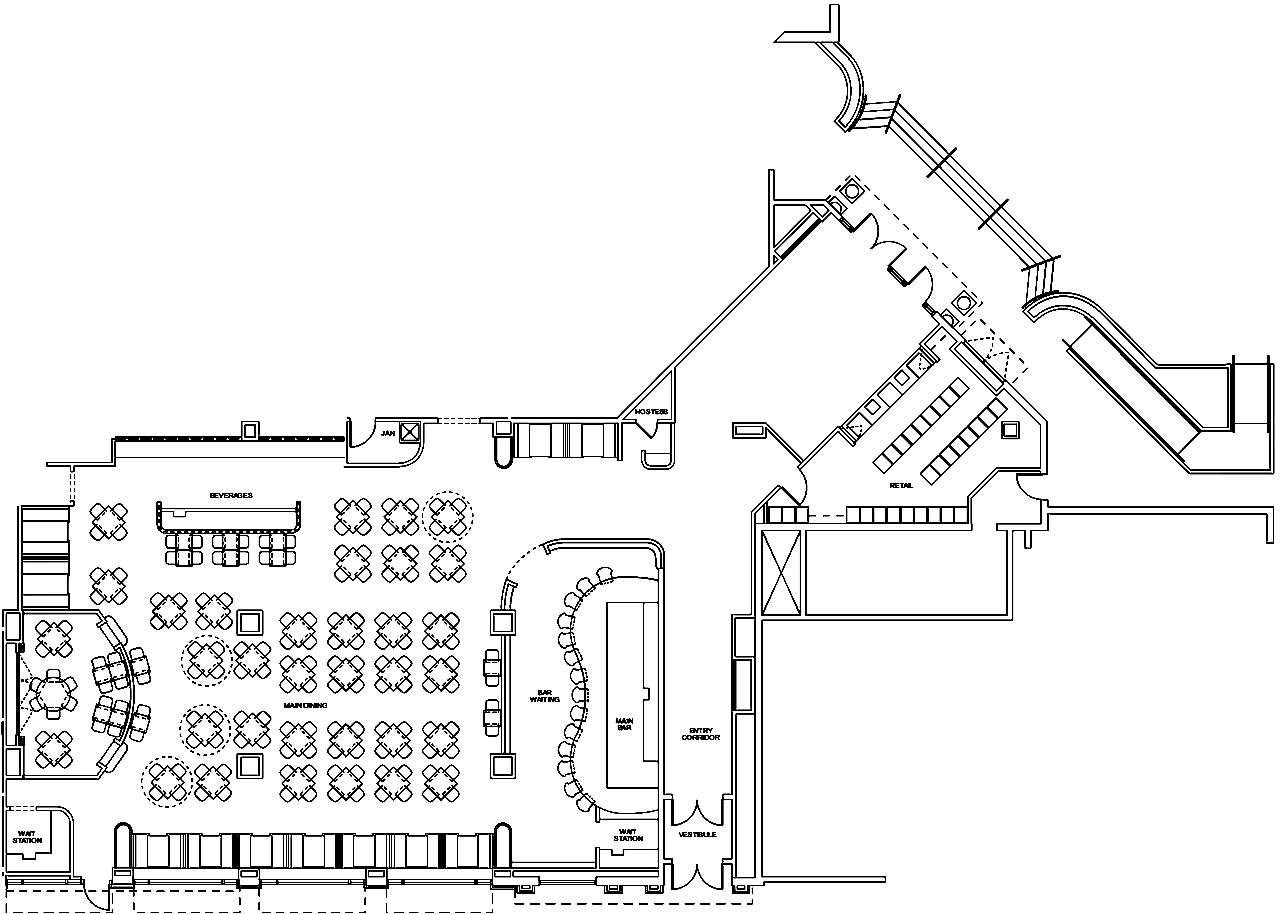
\includegraphics[width=1\textwidth]{img/hardrock-plan.png}
		\caption[Gebäudeplan Hardrock]{Gebäudeplan Hardrock Cafe, Atlantic City (Quelle: www.hardrock.com, 25.03.13)}
		\label{planHardrock}
\end{figure}

\subsection{Bar}
Die Bar dient als Warteschlange bis ein Tisch frei wird.
Servierpersonal an der Bar wird nicht berücksichtigt. Grund dafür ist eine fixe Anzahl Barpersonal.

Ziel ist es, dass an der Bar möglichst viele Plätze besetzt sind, weil diese Konsumenten konsumieren und Umsatz bescheren. Gleichzeitig sollte vor der Türe die Schlange möglichst klein oder gar nicht existieren, damit niemand an der Kälte warten muss, bzw wieder geht. Die Wartezeit an der Bar sollte nicht mehr als ein bis zwei Drinks betragen, damit niemand wieder geht, bevor ein Tisch frei wird.
Drinklänge: ca. eine Viertelstunde.

\subsection{Tische}
Am Tischen werden ein bis drei Gänge gegessen -> Verteilfunktion.
Als erstes soll eine Simulation einfach gehalten werden:
Servierdüse kommt einmal und bedient -> belegte Ressource für best. Zeit -> Verteilfunktion.
Teller und Karte bringen soll erst in einem zweiten Schritt modelliert werden, je nach Zeit.
- In der Realen Welt bestehen die Tische aus zweiertischen und die ankommenden Gruppen müssen auf Vielfache von Zweierplätzen aufgeteilt werden. Dabei kann es zu leeren Plätzen kommen. Der Einfachheit halber soll dies nicht berücksichtigt werden in der Simulation.
- Die Plätze werden fix gewählt anhand des Beispiels von Atlantic City. -> 250 Plätze

\subsection{Küche}
Erster Schritt: Keine Küche, nur bestimmte Wartezeit bis Essen fertig+gebracht.
Verschiedene Köche, die pro Essen / Gang eine Bestimmte Zeit gebunden sind -> Verteilfunktion.
Essen ist eine Ressource.

Anschliessend kehren die Gäste nach Hause zurück und der Tisch wird frei für neue Gäste.
Optional könnten einige Gäste erneut an die Bar zurückkehren.


\section{Warum soll Simuliert werden?}
\begin{itemize}
	\item Gebäudebau: Aus Kostengründen ist es nicht möglich einen Prototyp zu bauen
	\item Ist das Gebäude einmal gebaut, so kann die Bar kann nachträglich nur mit grossen Kostenaufwänden vergrössert oder verkleinert werden.
	\item Das Szenario ist zu kompliziert zum Rechen, weil zu viele Variablen im Spiel sind.
	\item Testen durch Reallive-Simulation ist nicht möglich, weil Statisten beim Warten sterben würden, vom vielen Essen dick würden oder verhungern würden beim Warten auf die Bestellung. Möglicherweise würden Sie auch an der Bar zu viele Drinks nehmen und wären zu betrunken zum Tisch zu wechseln.
\end{itemize}

\section{Objectives}
\begin{itemize}
	\item Vor der Türe:
		\begin{itemize}
			\item Queue: Ankommende Gäste lim(0)
		\end{itemize}
	\item Küche
		\begin{itemize}
			\item Agents: Köche
		\end{itemize}
	\item Bedienung
		\begin{itemize}
			\item Agents: Kellner, Tellerbringer
		\end{itemize}
	\item Bar
		\begin{itemize}
			\item Queue: Anzahl Warteplätze
		\end{itemize}
	\item Tische
		\begin{itemize}
			\item Ressourcen: Anzahl Plätze
		\end{itemize}
\end{itemize}


\section{Fragestellungen}
Ziel ist die Gewinnmaximierung durch gute Auslastung. Als gute Auslastung wird 75\% Utilisation angenommen.
\subsection{Grösse der Bar}
\textbf{Wie viele PLätze muss die Bar bieten, damit fast keine Gäste an der Kälte vor dem Eingang warten müssen und die mittlere Aufenthaltszeit an der Bar ein bis zwei Drinks nicht übersteigt?} \\
Als Länge für einen Drink soll 15-20 Minuten angenommen werden.


\subsection{Benötigtes Personal}
\textbf{Wie viel Servierersonal und wie viele Köche braucht es, damit die Mittlere Aufenthaltszeit am Tisch bei ca. 1.5 Stunden liegt?} \\


\section{Spezifikationen}
Gearbeitet wird mit Fiktiven Daten, ausgenommen die Anzahl der Plätze im Saal. Diese werden vom Hardrock Atlantic City übernommen.

\subsection{Variable Grössen}
Es sollen verschiedene Szenarien simuliert werden. Die dazu benötigten Grössen sollen Variabel sein:
\begin{itemize}
	\item Queuelänge
	\item Anzahl Servierpersonal
	\item Anzahl Köche
	\item Gruppen mit unterschiedlichen Anzahlen von Gästen
\end{itemize}

\subsection{Resultatgrössen}
Durch die Simulation sollen die \textbf{Aufenthaltszeit in der Queue}, die \textbf{Dauer des Aufenthaltes am Tisch}, die \textbf{Gesammtaufenthaltsdauer im Restaurant} und die \textbf{Auslastung der Agenten} ermittelt werden

\subsection{Zusatzprojekt (optional)}
In einem weiteren Projekt kann die Simulation ausgebaut werden verfeinert werden, indem weitere Parameter hinzugefügt werden und detailierter Daten erhoben werden:
\begin{itemize}
	\item Anzahl Personal an der Bar
	\item Kochzeit genauer simulieren, Simulation unterschiedlicher Kochzeiten für unterschiedliche Gänge
	\item Anzahl Tellerbringer
	\item Gruppen müssen zusammen an einem Tisch untergebracht werden
\end{itemize}


\chapter{Simulation}


\chapter{Auswertung}


\listoffigures


\chapter{Materialnachweise}
\section{Titelblatt}
\begin{tabularx}{\textwidth}{|Xlr|} % Versionstabelle, Rahmen links und rechts
		\hline
		Logo Hardrock & www.hardrock.com & 25.03.2013 \\
		\hline
\end{tabularx}

\end{document}
